\chapter{RESULTS AND DISCUSSION}

\paragraph\
The following section describes results obtained by performing the proposed test plan and the \acs{GDPR} readiness.

\section{\acs{IR} features test results} %YET TO FILL 
Due to access limitations, it was not possible to test Amazon Textract and Google Cloud Natural Language. The access for IBM Watson had some issues as it was old (Department had the access for over a year) and the credentials (API keys and URL) were not valid anymore to perform testing of the features in the service. Hence, testing was only done on Microsoft Azure.\\

The Evaluation Matrix \ref{section:matrix} after testing is as below:

\begin{table}[h]
\caption{Evaluation matrix} 
\begin{center}
   
  \begin{tabular}{| p{2.7cm} || p{2.7cm} | p{3.5cm} | p{2.12cm} | p{3cm} | p{1.9cm} |}
   
\hline
 \textbf{Service \hspace{1cm} Provider} & \textbf{\acs{IBM} Watson \acs{NLU}} & \textbf{Microsoft Azure Cognitive \hspace{1cm} Services} & \textbf{Amazon \hspace{0.3cm} Textract} & \textbf{Google Cloud Natural \hspace{1cm} Language} & \textbf{Datasets}\\ \hline \hline 
 
     \acs{PII} detection & Not available & Available & No access & No access & Dataset-3\\ [10pt] \hline
     Entity \hspace{0.2cm} Recognition & Available & Available & No access & No access & Dataset-3\\ \hline
     Sentiment Analysis & Available & Available & No access & No access & Dataset-4 \\ \hline
     Summarization & No clarity on availability & Available & No access & No access & Sample texts\\ \hline
     Classification & Unable to test & Unable to test & No access & No access & Not \hspace{1cm} applicable\\ [10pt] \hline 
     (\acs{OCR}) Optical Character Recognition & Not available & Available & No access & No access & Dataset-1, Dataset-2 \\ \hline
     Free trial for users & Not available & Available for 30 days & Not \hspace{1cm} available & Not available & Not \hspace{1cm} applicable\\ [15pt] \hline
     Documentation to use the \hspace{1cm} service & Available & Available & Available & Available & Not \hspace{1cm} applicable\\ \hline
     
\end{tabular}                          
\end{center}
\end{table}
\clearpage

\textbf{Azure Testing:}
\begin{itemize}
    \item \uline{Testing \acs{PII} and \acs{NER} on Dataset-3 (\ref{subsection:data3})}\\
    Azure Cognitive Services Language Studio for free tier resource allowed only an input limit of 5000 characters and the input could be either typed or uploaded in the form of a 'txt' file only \ref{azinputlimitation}. As our dataset was in the form of a 'csv' file; it was first converted to a 'txt' file (a snippet of the text file is in Appendix \ref{aztextinputfile}) and uploaded. The input was trimmed to the first 5000 characters of the file and was processed. Tried to upload the 'csv' file directly and it uploaded without any error, but again trimmed the content to the first 5000 characters and displayed it in the input box. A snippet of the input text box can be seen in Figure \ref{d3piiin} and a glimpse of the identified list of \acs{PII}s are shown in \ref{d3piiout}. A snippet of results obtained for identifying entities can be seen in \ref{d3nerout}. Along with fields like \textit{PersonType}, \textit{Person}, \textit{Date}, it has also identified \textit{Currency}, \textit{Location}, \textit{Quantity} and so on in \acs{NER}.
    \begin {figure}[h!h]
        \centering
        \adjustbox{frame}{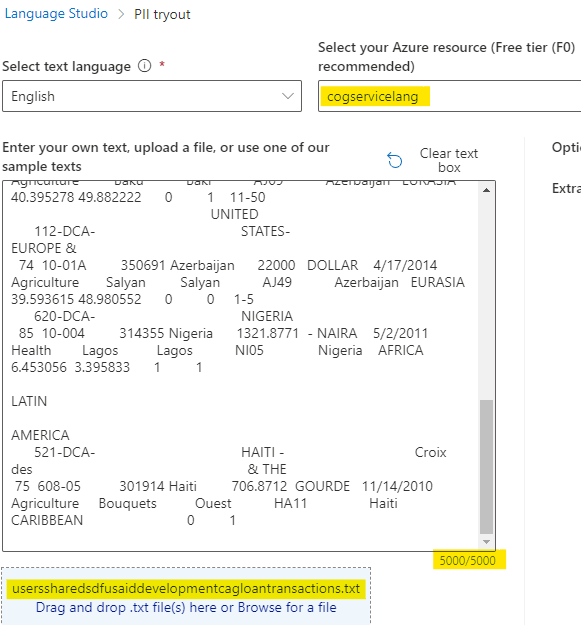
\includegraphics[scale=0.85]{images/Chapter5/pii_input_d3.png}}
        \caption{Input screen for \acs{PII} detection feature}
        \label{d3piiin}
        \end {figure}
    \begin {figure}[h!h]
        \centering
        \adjustbox{frame}{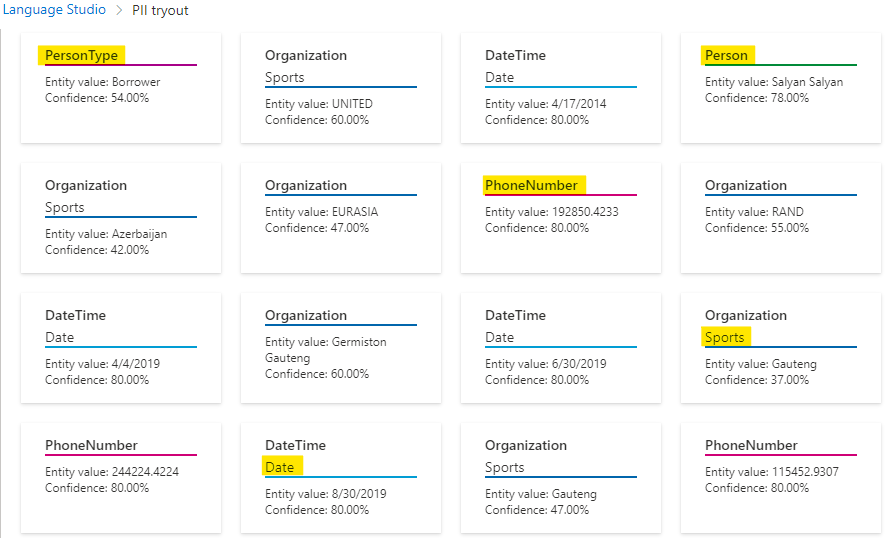
\includegraphics[scale=0.684]{images/Chapter5/pii_output_d3.png}}
        \caption{Result screen for \acs{PII} detection feature}
        \label{d3piiout}
    \end {figure}
    \begin {figure}[h!h]
        \centering
        \adjustbox{frame}{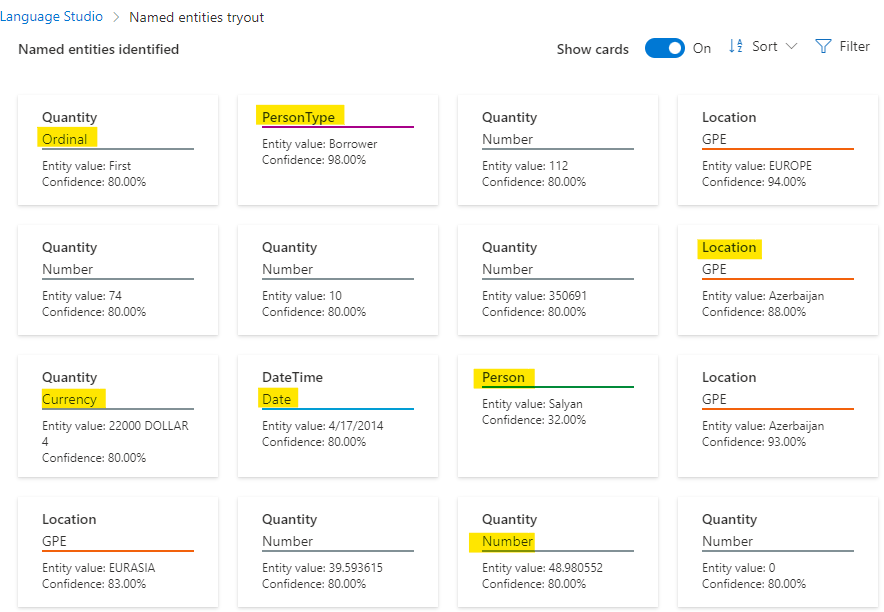
\includegraphics[scale=0.685]{images/Chapter5/ner_output_d3.png}}
        \caption{Result screen for \acs{NER} feature}
        \label{d3nerout}
    \end {figure}
    \newpage
    \item \uline{Testing Sentiment analysis on Dataset-4 (\ref{sentidataset})}\\
    Though there were two datasets for sentiment testing, Dataset-2 (\ref{subsection:data2}) was an image dataset and hence could not be used in Azure Language Studio. So Dataset-4 was added to the dataset collection and used for testing. As it accepted inputs better in text format, converted the 'csv' file into 'txt' and split each tweet (without the label) into a single text file to provide input for the Sentiment analysis feature in the language studio. Added about 7 text files to stay within the 5000 characters limit. But when processed, it only read the first text file as input and provided analysis for it. Figure \ref{d4sentiin} shows a snippet where all 7 text files are uploaded but only the tweet from the first text file is taken as input. It accurately classified the sentiment of the input document as 'Negative'. Results can be seen in Figure \ref{d4sentiout}.
    \begin {figure}[h!h]
        \centering
        \adjustbox{frame}{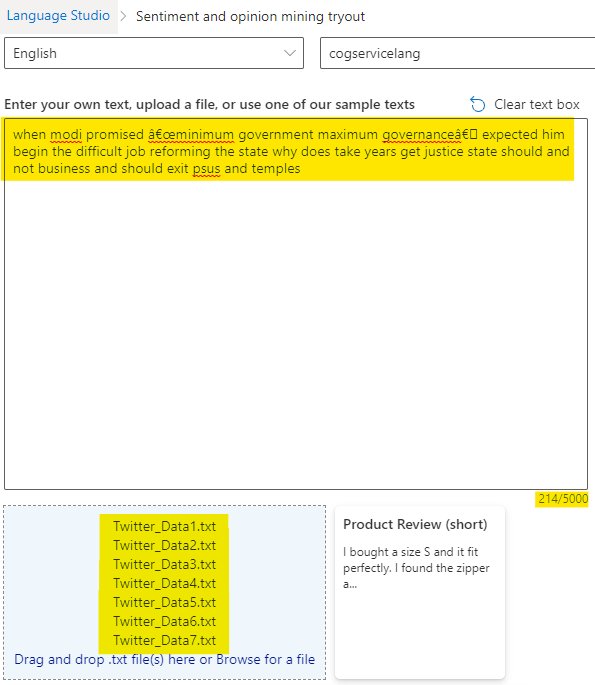
\includegraphics[scale=0.859]{images/Chapter5/senti_input_d4.png}}
        \caption{Result screen for \acs{NER} feature}
        \label{d4sentiin}
    \end {figure}
    \begin {figure}[h!h]
        \centering
        \adjustbox{frame}{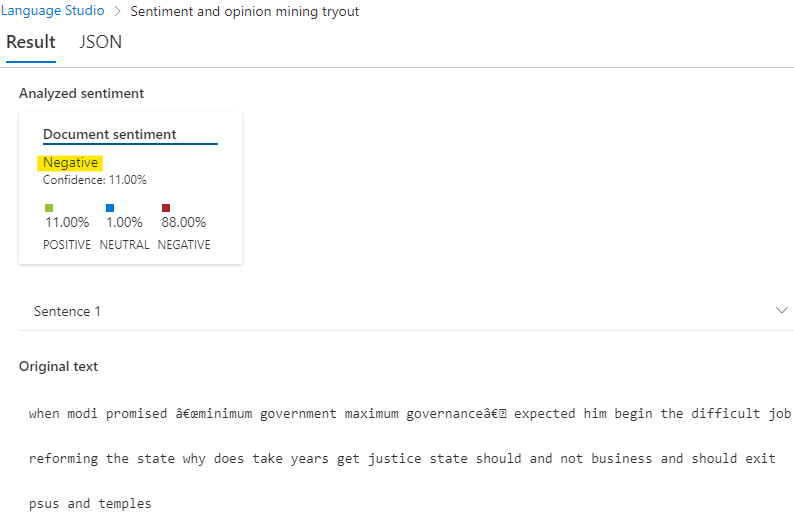
\includegraphics[scale=0.7]{images/Chapter5/senti_output_d4.png}}
        \caption{Result screen for \acs{NER} feature}
        \label{d4sentiout}
    \end {figure}
    \item \uline{Testing \acs{OCR} on Dataset-1 (\ref{textocrdataset}) and Dataset-2 (\ref{sentiocrdataset})} \\
    As \acs{OCR} was not present in Language Studio, uploaded dataset-1 (25,000+) image files into Azure blob storage to connect it to the Azure Cognitive services as described in Chapter-4. It took about 30-35 minutes to upload all the image files to the storage container. A snippet is added in Appendix \ref{ocrd1upload}. Repeated the process for dataset-2 which had comparatively lesser files (239). For this upload, it took about 30-40 seconds. After creating an index and running queries, the texts were extracted from input files. 
    \begin {figure}[h!h]
        \centering
        \adjustbox{frame}{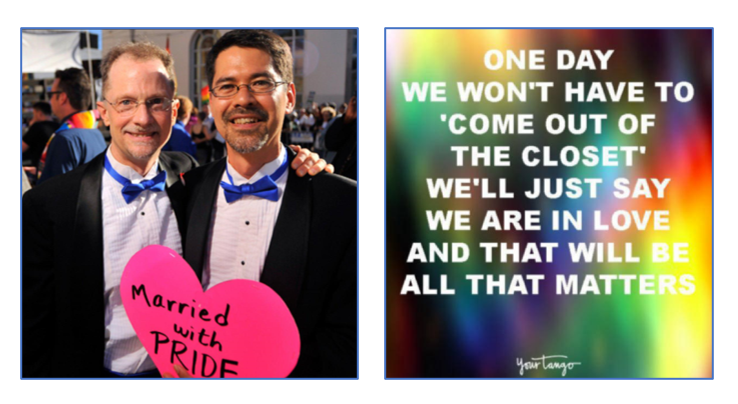
\includegraphics[scale=0.6]{images/Chapter5/senti_ocr_input_d2.png}}
        \caption{Example input image files for \acs{OCR} feature}
        \label{d2sentiocrin}
    \end {figure}
    \newpage
     Results for \acs{OCR} on dataset-2 are shown in Figure \ref{d2sentiocrout}. From 239 input files, the \textit{keyphrases} list along with the entire \textit{text} extracted from one of the image files. The author (randomly) considered another input image file to check if the text from it was also rightly extracted but couldn't find the text being extracted from it. Input images for both these results are shown for reference in Figure \ref{d2sentiocrin}. The left side is the input image for which the text was not extracted as seen in Figure \ref{d2sentiocrout2}; the right is the input image for which it was extracted.
    \begin {figure}[h!h]
        \centering
        \adjustbox{frame}{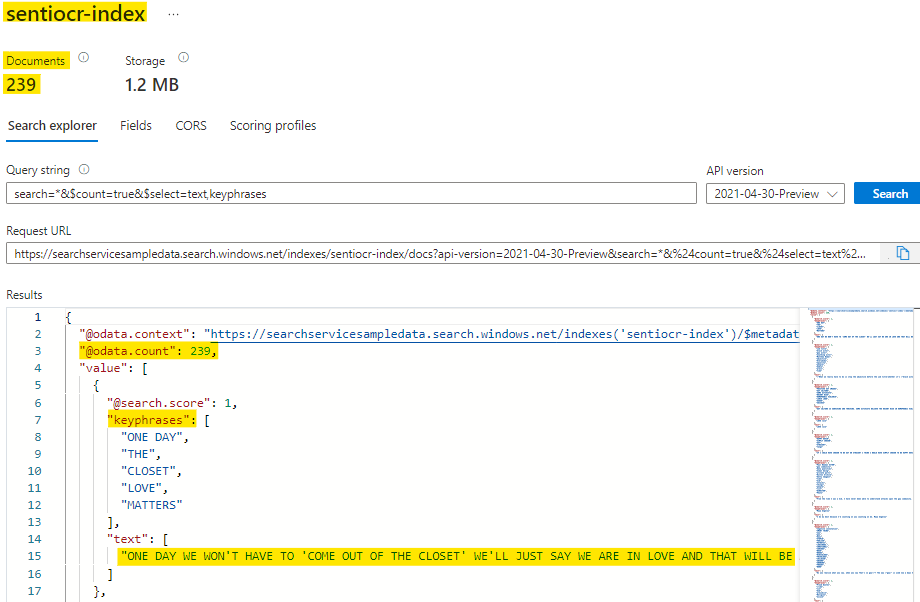
\includegraphics[scale=0.61]{images/Chapter5/senti_ocr_output2_d2.png}}
        \caption{Result screen for \acs{OCR} features extracted of an example image}
        \label{d2sentiocrout}
    \end {figure}
    \begin {figure}[h!h]
        \centering
        \adjustbox{frame}{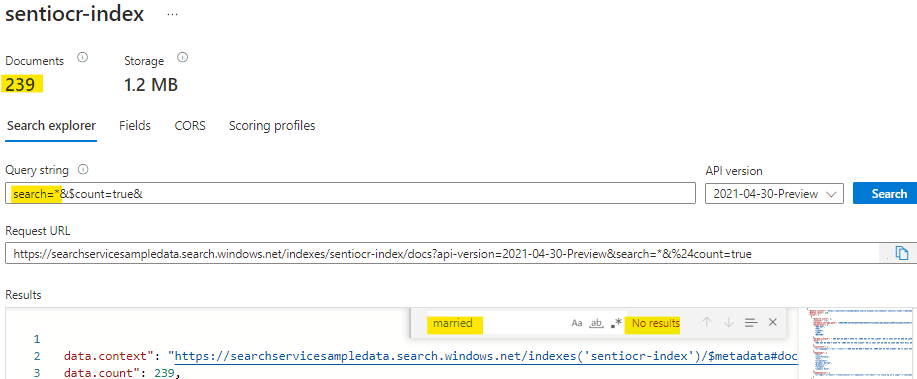
\includegraphics[scale=0.645]{images/Chapter5/senti_ocr_output3_d2.png}}
        \caption{Result screen for \acs{OCR} feature where text was not extracted}
        \label{d2sentiocrout2}
    \end {figure}
   \newpage
   From Figure \ref{d2sentiocrout2}, it is clear that the text in the input file (left image in Figure \ref{d2sentiocrin}) was not extracted. The author searched for the text in the image "Married with PRIDE" and there were no results. Shortened the search term to just "married" and still there were no results. Tried other search terms like "PRIDE" and all the above mentioned with change in casing and still no results were found. There were more fields returned for query {\texttt{'search=*\&\$count=true'}}
   and not just \textit{keyphrases} and \textit{text}. A whole set of fields returned can be seen in Appendix \ref{sentiocrres}.\\
   Results for \acs{OCR} on dataset-1 are shown in Figure \ref{d1stextocrout}. This shows results of query\\ {\texttt{'search=*\&\$count=true\&\$select=text,masked\_text,pii\_entities'}}. \\ While creating this index, \textit{pii\_entities} was selected too and it is seen that they are identified as well. In \textit{masked\_text} field we can see the entire text but with \acs{PII} information obscured. The input image is shown for reference in Figure \ref{d1stextocrin}. But it was noted that only 36 documents were uploaded instead of 25,199 files (\ref{ocrd1upload}). In Appendix \ref{item:textocrresults} snippets of results showing all the fields displayed in results are shown.
   \begin {figure}[h!h]
        \centering
        \adjustbox{frame}{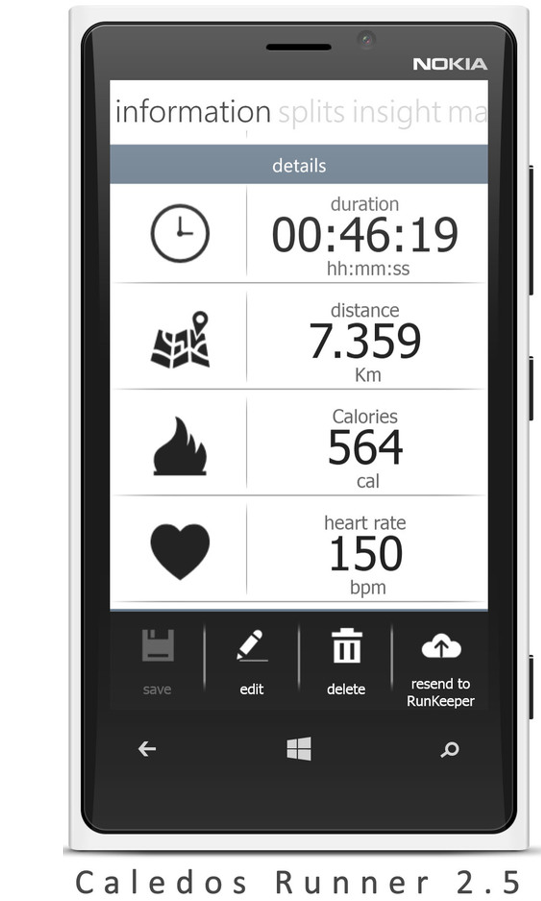
\includegraphics[scale=0.56]{images/Chapter5/text_ocr_input_d1.png}}
        \caption{Result screen for \acs{OCR} feature where text was not extracted}
        \label{d1stextocrin}
    \end {figure}
    \begin {figure}[h!h]
        \centering
        \adjustbox{frame}{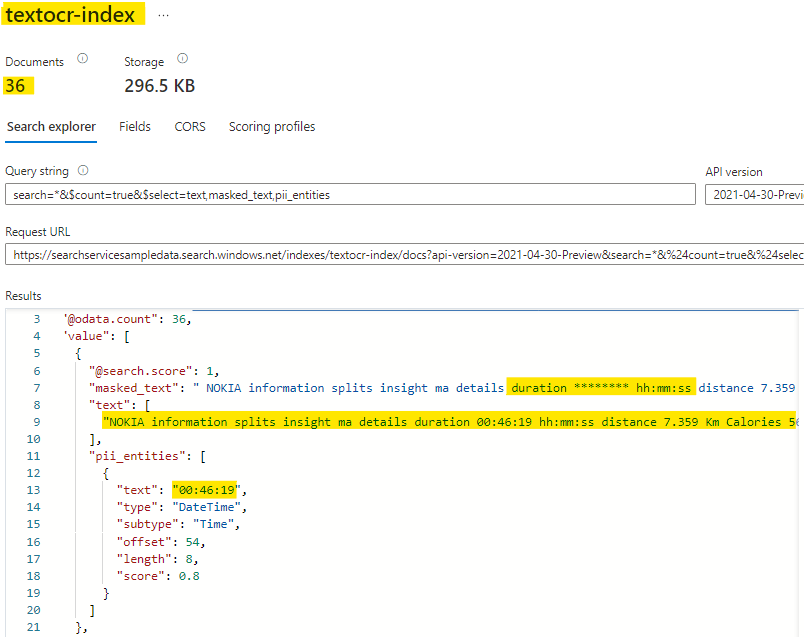
\includegraphics[scale=0.785]{images/Chapter5/text_ocr_output_d1.png}}
        \caption{Result screen for \acs{OCR} features extracted of an example image}
        \label{d1stextocrout}
    \end {figure}
\end{itemize}

\textbf{IBM Testing:}
\begin{itemize}
    \item \uline{Testing \acs{PII}, \acs{OCR} and summarization}\\
    These features were not available in IBM Watson \acs{NLU} service. Figure \ref{ibmnotsupported} is a snippet from the 'Getting started' tutorial video of Watson \acs{NLU} \cite{ibmstarter} after creating the Watson \acs{NLU} resource instance. The snippet displays a list of the features available in this service and \acs{PII}, \acs{OCR}, and Summarization are not in it.
    \begin {figure}[h!h]
        \centering
        \adjustbox{frame}{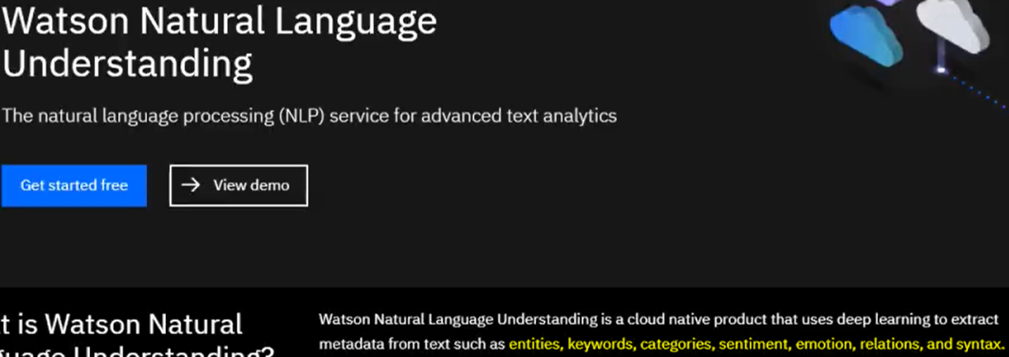
\includegraphics[scale=0.56]{images/Chapter5/waton_not_supported.png}}
        \caption{Features available in IBM Watson \acs{NLU}}
        \label{ibmnotsupported}
    \end {figure}
    \item \uline{Testing \acs{NER}, classification and sentiment analysis}\\
    There was an issue with API keys and URL as the attempt was resulting in a 401 error. Snippet is shown in Figure \ref{ibm401error}. Tried to manually access the URL and entered credentials for IBM Watson and it was the same error as seen in Figure \ref{ibm401error1}. The website, to which the error directed did not provide any information or workaround. There was no update option available on the IBM Catalog page.
    \begin {figure}[h!h]
        \centering
        \adjustbox{frame}{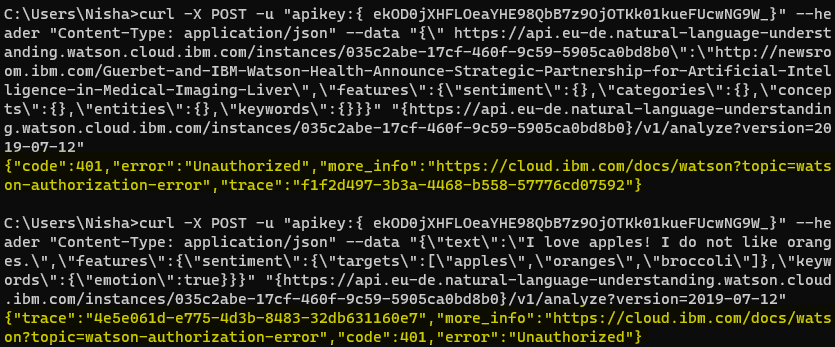
\includegraphics[scale=0.67]{images/Chapter5/watson_curl_error.png}}
        \caption{401 Error while trying to analyze features of Watson \acs{NLU}}
        \label{ibm401error}
    \end {figure}
    \begin {figure}[h!h]
        \centering
        \adjustbox{frame}{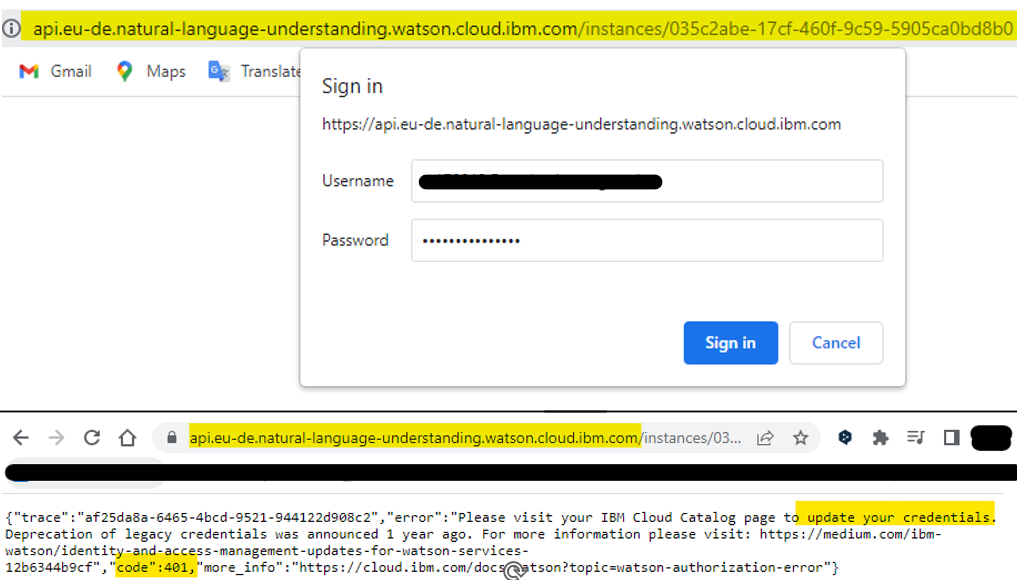
\includegraphics[scale=0.54]{images/Chapter5/watson_curl_error_manual.png}}
        \caption{Same 401 error appeared when tried the URL manually}
        \label{ibm401error1}
    \end {figure}
\end{itemize}

\clearpage
\newpage
\begin{itemize} 
    \item \underline{IBM Watson:}
    The \textbf{first} feature \acs{PII} detection was not available as part of Watson \acs{NLU} (Figure \ref{ibmnotsupported}). Upon further research, it was found that this feature could be added to the project or application by creating an instance of IBM's other service IBM Watson Studio. However, it was not available in the service tested during the course of this thesis.\\
    The \textbf{second} feature entity extraction in IBM when tested, identified 14 entities mentioning the type and confidence for each. There was no option to identify sub-type of entities. It identified most of the entities correctly but a few were skipped ('Chicken parmigiana dish', 'card', 'validation') and one was classified as type \textit{phone number} while it was actually a social security number. So it was not fully accurate but it did identify basic entities.\\
    Sentiment analysis, the \textbf{third} metric from the evaluation matrix was also available in IBM Watson \acs{NLU}. It accurately classified the input document as a 'Positive' class with confidence of '78\%'. It also provided sentiment classification and scores for a few keywords but did not have sentence-level analysis. Tested on a neutral sentiment where the sentiment was not present or at least not very obvious. IBM classified it as positive with a confidence of 72\% as seen in Appendix \ref{item:neutral}.\\
    The \textbf{fourth} feature summarization was not present in the demo portal of Watson \acs{NLU} but the resources \cite{watsonnlu} specified that this feature was available as part of Watson \acs{NLU} subscription but it had experimental written beside this feature \cite{ibmsumm}. There was no clear information about what the 'experimental' beside this feature indicated. When created Watson \acs{NLU} this feature was not available for testing and is not part of the official get started tutorial video either as seen in Figure \ref{ibmnotsupported}.\\
    The \textbf{fifth} feature classification was not present in the demo portal of Watson \acs{NLU} but the resources \cite{watsonnlu} specified that this feature was available to users as part of Watson \acs{NLU} subscription. Unfortunately, this could not be tested.\\
    The \textbf{sixth} feature \ac{OCR} was not present in the demo portal of Watson \acs{NLU}.\\
    In IBM Cloud API Docs \cite{watsonnlu}, it gives the users a detailed description of what each feature is and examples of how to use it. \cite{ibmstarter} has a short tutorial introducing \acs{NLU} \acs{API} providing examples and links to additional resources. \cite{ibmdemo} allows the user to test the features with already provided sample text inputs and also provides an option for users to test it on a custom piece of text or a \acs{url} link. IBM also has an \acs{FAQ} section \cite{ibmfaq} in the Watson \acs{NLU} page which has answers to many details including the usage of various (free/lite) plans and storage of user data and pricing plans. IBM Developer site has various tutorials in fields like \acl{ML}, \acl{AI}; one interesting tutorial was on sentiment analysis using IBM Watson natural language processing \cite{ibmref1}. Users can find many tutorials in this section for entity extraction \cite{ibmee}, text classification \cite{ibmtc}, and so on.
    
    \item \underline{Microsoft Azure:} 
    In section \ref{section:impl}, testing of the features is described in detail with snippets from testing. It can be stated that the \textbf{first} metric \acs{PII} detection feature worked well as it not only identified all the sensitive personal information along with mentioning what kind of information it was; but also provided the option to display the document after obscuring the identified \acs{PII} data in it. But testing results showed that it was not completely accurate. In one of the examples, as seen in Figure \ref{piioutput}, it failed to identify the social security number as a \acs{PII} which could serious trouble in real-life applications.\\
    The \textbf{second} metric Entity recognition identified about 19 entities during testing. All the identified entities were done so with the types and subtypes as seen in Figure \ref{piiogtext}. It did not identify the social security number '123-45-6789' as a single identity but, it instead identified '123', '45', and '6789' as 3 separate entities of type \textit{number}. \\ 
    The \textbf{third} feature sentiment analysis was also available in Azure Cognitive Services for Language. It provided sentiment (positive, negative, natural) classification for the document as well as each sentence in the document. It also mentioned the confidence for each of the sentiments and then classified the text into the sentiment class with the highest confidence. In one of the examples however, it happened that though the negative sentiment had a confidence of 99\%, the other two sentiments had 0\%, and the statement was classified as negative but with 0\% confidence. This was weird too as the summation of all 3 sentiments had to be a total of 100\% which was not in this case and also the confidence of the statement was shown as 0 instead of 99\%. This is visible clearly in Figure \ref{saoutput}. Tested this feature for the same neutral statement (used to test for IBM) to compare its performance against IBM, it classified the statement as 'Neutral' with 97\% confidence as seen in Appendix \ref{item:neutral}\\
    The \textbf{fourth} feature Summarization feature was available for texts and conversations with different options for each. There were no inconsistencies found during the testing of this feature. Test results are shown in \ref{summzresp} and \ref{summzresp2}.\\
    The \textbf{fifth} metric was classification of text; it required the user to create a project and add language resource to proceed further. There was an issue at this stage and this feature could not be tested. Details of this situation are described in Appendix \ref{item:tcfeature}.\\
    The \textbf{sixth} feature \acs{OCR} was not available in Language Studio and was tested in Azure Cognitive Search service. The performance was mixed as it was seen above that in one of the images, it extracted all the text accurately \ref{d2sentiocrout} and for another randomly picked input image, the text was not extracted \ref{d2sentiocrout2}. With \textit{pii\_entities enabled}, another field \textit{masked\_test} was shown where the extracted text was shown after obscuring the \acs{PII} information \ref{d1stextocrout}.\\
    The documentation for Microsoft Azure was easily accessible in the Microsoft Learn portal. Few of the useful links are \cite{azdocs1}, \cite{azdocs2}, \cite{azdocs3}, \cite{azdocs4}. There were also useful tutorials to get started with Azure Cognitive Search Service in links \cite{azdocs}, \cite{azuretutorial} but there were no tutorials for 'Azure Cognitive Service for language'.
    
    \item \underline{Amazon Textract:} Amazon only had the '\acs{AWS} educate' option as a free subscription to learn about various services provided by Amazon but it was a limited set of options and did not have Textract in it. And after having a long call with their support team it was confirmed that there was only one way to get access to Textract and that is to provide a payment method while creating the login account. So unfortunately, testing of this cloud service provider for \acs{PII} detection, entity recognition, sentiment analysis, \acs{OCR}, summarization and text classification could not be done in this thesis. The availability of documentation in the form of instructions or tutorials was checked to evaluate the last metric. Amazon Docs published a full guide \cite{awspdf} explaining what is Textract and how to use it, best practices, explaining each of the \acs{API}s, and link to tutorials \cite{awstut}. They also had a detailed developer's guide on Github \cite{awsgit}. On the AWS website, there is a dedicated page for \acs{FAQ}s on Amazon Textract \cite{awsfaq} \cite{awstextarct}. 
    
    \item \underline{Google Cloud:} Google provided 200 credits for users who register as students and these credits are valid for one year since the registration. Google Cloud Natural Language had guides and learning paths to use the services with qwiklabs with temporary user access. But with this, there is limited (time) and temporary access which was also only \ac{CLI} and not \ac{UI} based as shown in their preview video \cite{gcpreviewvideo} which is linked in their lab tutorials \cite{gcqwiklab}.
     It was necessary to provide payment details in order to get full access to Google Cloud Natural Language and hence the testing of the first five metrics was not possible due to lack of access.
     Testing of a few statements was possible but could not do the testing for a large set of data files; this was possible in the paid subscription models. Although Google did have sufficient documentation and qwiklabs as tutorials for users to try the features; these tutorials had very limited access (both in terms of time and features). Hence it was possible to only get a glimpse of what would be available when a subscription is purchased. Few of the tutorial and documentation guides for Google Cloud Natural Language can be found in \cite{gcdocs1} \cite{gcdocs2}, \cite{gcdocs3}, \cite{gcinsights} and \cite{gcqwiklab}.
\end{itemize}

\section{\acs{GDPR} readiness}
The \acs{GDPR} readiness of these services are discussed in this section. As there is no public list of \acs{GDPR} compliant/\acs{GDPR} certified companies, in this section, all relevant information is gathered that was published in official documents and blogs and is discussed briefly while mentioning the source of the information. Companies can obtain \acs{GDPR} certification however, it is voluntary as clearly stated in article 42 of \acs{GDPR} \cite{gdprart42}. Companies can assess themselves with the checklist \cite{gdprchecklist} provided to evaluate if their policies are up-to-date and make certain changes if needed to comply with the \acs{GDPR}.

\begin{table}[h]
\caption{GDPR compliance} 
\begin{center}
   
  \begin{tabular}{| p{2.8cm} || p{2.7cm} | p{3.5cm} | p{2.1cm} | p{2.9cm} |}
   
\hline
 \textbf{Service Provider} & \textbf{\acs{IBM} Watson \acs{NLU}} & \textbf{Microsoft Azure Cognitive \hspace{1cm} Services} & \textbf{Amazon Textract} & \textbf{Google Cloud Natural \hspace{1.5cm} Language}\\ \hline \hline 
 
     \acs{GDPR} \hspace{1.3cm} Certificate & Not available & Not available & Not \hspace{1.5cm} available & Not available\\ \hline
     ISO 27018 \hspace{1.3cm} Certificate & Available & Available & Available & States available but no access\\ \hline
     \acs{FAQ} for \acs{GDPR} \hspace{1.3cm} Compliance & Available & Available & Available & Available\\ \hline
     Live tracking of customer data & Not available & Available & Not \hspace{1.5cm} available  & Not available\\ \hline 
     
\end{tabular}                          
\end{center}
\end{table}

\begin{itemize}
    \item \underline{\acs{GDPR} readiness in \acs{IBM} Watson:}    
    
    The main pillars of data privacy and security strategy for \acs{IBM} Watson are Governance, Risk, and Compliance (GRC) \cite{ibmgdpr}. \acs{IBM} claims \cite{ibmgdpr3} to have a framework set up to ensure all its products and services comply with \acs{EU}'s \acs{GDPR} (came into effect on May 2018). \cite{ibmgdpr} provides details on \acs{IBM} Cloud compliance especially for Watson services. It also provides a link to IBM's \acs{ISO} 27018:2014 certificate \cite{ibmisocert}. Upon research, it was also found that \acs{IBM} Enterprise and Technology has the \acs{ISO} 27018:2019 certificate \cite{ibmisocert2}. \ac{ISO} 27018 certifies adherence to fulfilling the requirements of data protection and security law; focusing mainly on personal data in cloud \cite{isocert}. In the document, it mentions that \acs{IBM} was proactive with data security and was already \acs{GDPR} compliant in May 2018. The second half of the document lists answers to numerous  \ac{FAQ}s of various categories like Data Privacy, Compliance, Security, Encryption, Vulnerability Management, and Security Management to help understand the data security measures of \acs{IBM} and give a sense of transparency. Figure \ref{ibmgdpr} is a snippet of one such \acs{FAQ}  from the document \cite{ibmgdpr} mentioning the compliance.
    
    \begin {figure}[ht]
    \centering
    \adjustbox{frame}{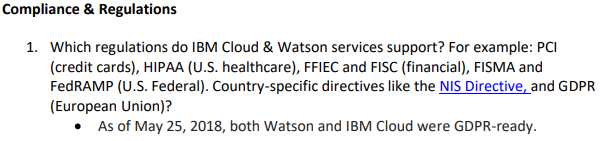
\includegraphics[width=0.78\textwidth]{images/Chapter5/ibm_gdpr.png}}
    \caption{Compliance and Regulations}
    \label{ibmgdpr}
    \end {figure}
    
    \acs{IBM} also provides assistance to its clients in their journey to \acs{GDPR} readiness, under the '\acs{IBM} \acs{GDPR} Framework' \cite{ibmgdprservice}. The framework has five phases: Assess, Design, Transform, Operate and Conform. With the help of this framework, \acs{IBM} aims to assist its clients to manage privacy and security efficiently and support the clients in their journey towards \acs{GDPR} readiness. In \cite{ibmgdpr2}, IBM's then (2017) Chief Privacy Officer Cristina Cabella stated that \acs{IBM} was already adapting internally to \acs{GDPR} guidelines for when it would come into effect in 2018.
    
    \item \underline{\acs{GDPR} readiness in Microsoft Azure:}
    
    Microsoft Azure also has \acs{ISO} 27018:2019 certificate \cite{azureisocert}. \cite{azurecompliance} is the Microsoft portal for all audit reports, certificates, and audit documentation. It has a specific portal \cite{azureservicetrustportal} for all the compliance certificates for Microsoft products. In \cite{azuregdpr}, it explains what is \acs{GDPR} briefly, the main terminologies needed to understand the regulations. It acts as a guide to information on what are the user's rights and duties when using Microsoft's products and services. The compliance and security measures in Microsoft Azure Cognitive Services in specifically are of interest as that is one of the services researched for testing in this thesis. In \cite{azuregdprcompliance}, Azure describes its customer data handling measures with respect to compliance, privacy, and transparency. A snippet from the site about transparency can be seen in Figure \ref{azuretransparency}. It even provides a live tracking \cite{azuredatamap} option for customers to view where their data if stored is currently at rest. 

    \begin {figure}[ht]
    \centering
    \adjustbox{frame}{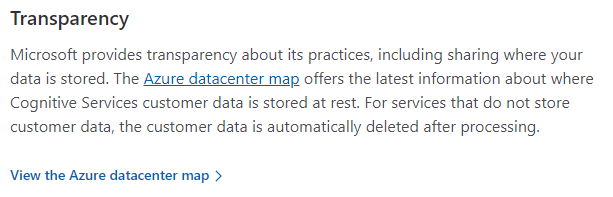
\includegraphics[scale=0.78]{images/Chapter5/Azure_data_transparency.png}}
    \caption{Data Transparency in Azure Cognitive Services}
    \label{azuretransparency}
    \end {figure}
    Like IBM, Microsoft also assists its clients to be \acs{GDPR} compliant. It has a four steps process to help the clients meet the \acs{GDPR} requirements. \cite{azuregdpr2} describes the four steps namely: Discover, Manage, Protect, and Report.
    %\vspace{1.5cm}
    
    \item \underline{\acs{GDPR} readiness in Amazon Textract:}

    Amazon Web Services has a website \acs{GDPR} center \cite{awsgdprcenter} where they share information with its customers about \acs{AWS}'s \acs{GDPR} compliance. It has details on how the customer has control over their customer data. For instance, \acs{AWS} lets the customers determine where their data is to be stored, which region geographically, and what kind of storage is to be used. It also provides a provision for customers to choose and manage their own encryption keys for \acs{AWS}'s data encryption methods for data at rest or in transit. Customers are also in control of who can access their data with the help of user group permissions and credentials. This site also \acs{FAQ} s on \acs{GDPR} where it gives customers a basic introduction to what is \acs{GDPR} and how \acs{AWS} incorporates the \ac{SCC}s  into \acs{AWS} \acs{GDPR}. \acs{SCC}s are \acs{GDPR} approved methods to transfer personal data to countries outside the \ac{EEA} whose activities are not subject to \acs{GDPR}. A snippet of one of the \acs{FAQ} s about the incorporation of \acs{SCC}s in \acs{AWS} \acs{GDPR} can be seen in Figure\ref{awsgdpr}.

    \begin {figure}[ht]
    \centering
    \adjustbox{frame}{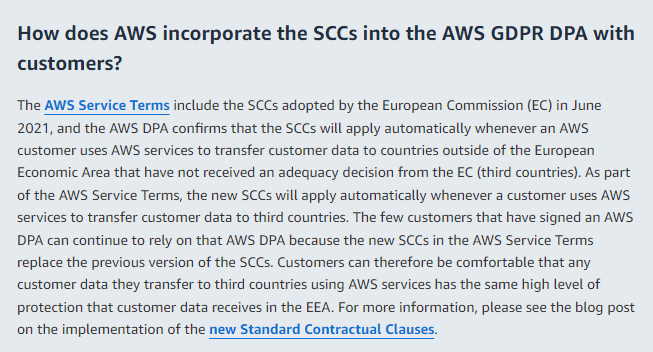
\includegraphics[scale=0.8]{images/Chapter5/aws_gdpr.png}}
    \caption{\acs{AWS} and \acs{GDPR} compliance}
    \label{awsgdpr}
    \end {figure}

   In \cite{awsgdprresp} \acs{AWS} talks about its roles as both data controllers and processors. It explains the role of the data processor in detail and explains how it has audits from third parties to ensure its security measures are intact and fix the issues if found. As an example, it also has a link to view the \acs{ISO} 27018:2019 certificate for \acs{AWS} \cite{awsisocert}. In the blog \cite{awsgdprresp} \acs{AWS} also provides recommendations to its customers on taking steps from their end to ensure the privacy and security of data with measures like \ac{MFA}, mandating the use of \acs{SSL}/\acs{TLS} encryption for communicating with services, setting user activity logging and so on.
    
    \item \underline{\acs{GDPR} readiness in Google Cloud:}

    Google Cloud has a public document named 'Google Cloud and the \ac{GDPR}' \cite{gcgdpr} in which it explains \acs{GDPR} and Google Cloud's commitment to comply with it. A snippet can be seen in Figure \ref{googlegdpr} below. In the document, Google explains in detail about their reliability, data processing agreements to comply with \acs{GDPR}, and security measures for communication with and between the services. It also explains about their Data deletion and retention policies. For instance, when a user provides Google with a full delete instruction, Google will then proceed to erase the confirmed data from all its system within the maximum duration of 180 days after confirming that there are no conflicts with any of the retention obligations. It also mentions under the 'International Data Transfers' section that they have data protection agreements to perform the data transfer while still complying with \acs{GDPR} even when data transfer involves countries outside the \acs{EU}.
    
    \begin {figure}[ht]
    \centering
    \adjustbox{frame}{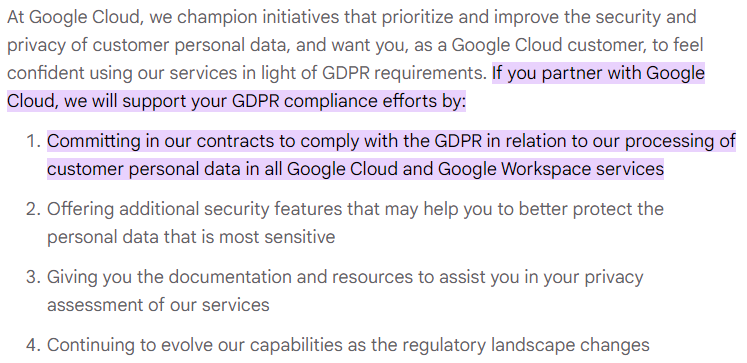
\includegraphics[scale=0.67]{images/Chapter5/google_gdpr.png}}
    \caption{Google Cloud \& the General Data Protection Regulation (GDPR)}
    \label{googlegdpr}
    \end {figure}

    In \cite{gcisoblog}, Google states that Google Cloud (along with Google Workspace, Chrome, and others) is \acs{ISO}/\acs{IEC} 27018 certified. Unlike the above cloud service providers, the compliance reports and certificates for Google Cloud are not available easily; they require an additional step to set up a Google Workspace account to be able to access them. In the blog a link is provided to their Compliance Manager \cite{gccompliancemgr} but upon reaching the site, it prompts the user to sign in with their Google Workspace credentials in order to be able to view or download any kind of reports or certificates. The creation of this account (both business edition and education/non-profit edition) required the user to have a domain or purchase one. As the author didn't have a domain and could not purchase one (which was only possible at a certain cost) had no other way to create the account and had to discontinue the process. Hence, it was not possible to view the \acs{ISO} certificate or provide a link for one. It was only possible to provide the link to the compliance manager \cite{gccompliancemgr} which would allow anyone with a Google Workspace account to view the certificates and assess them. Screenshots (\ref{gcworkaccs} and \ref{gcworkaccdomains}) during the account creation by the author are added in Appendix for reference.
    
\end{itemize}